\documentclass[25pt, a3paper,portrait]{tikzposter} %orientation options: portrait, landscape
\usepackage[utf8]{inputenc}

\title{ \textbf{United College Of Engineering \& Research}}
\author{Naini Prayagraj Uttar Pradesh \\
Department of Computer Science Engineering And Information Technology\\
\textbf{\underline{CRIME GLANCE}} \\
\bold{Session: 2022 - 2023}
}
\institute{Under the Guidance: MR. BHANU PRATAP RAI }

\usepackage[backend=biber, style=numeric, sorting=none, locallabelwidth]{biblatex}
\bibliography{ref}

\usetheme{Rays} % Options: Default, Simple, Basic, Rays, Wave, Envelope, Board, Autumn, Desert

\graphicspath{Images/}

%import necessary packages
\usepackage{blindtext}
\usepackage{graphicx}
\usepackage{caption}
\usepackage{subcaption}
\usepackage{comment}
\usepackage{amsmath,amssymb}

\begin{document}

\maketitle

\node[anchor=west, xshift = -1 cm ] at (TP@title.west) {
\includegraphics[width=10cm]{aktu.png}}; %left logo, comment out if unnecessary
\node[anchor=east, xshift = 1 cm] at (TP@title.east) {
\includegraphics[width=9cm]{ucer1.png}}; %right logo, comment out if unnecessary

\block{Abstract}
{
    The alarming increase in crime rates in recent years has posed serious problems for communities all around the world. The rise in criminal activity has been attributed to a number of factors, including socioeconomic inequalities, drug misuse, insufficient law enforcement resources, and new criminal methods, needing immediate action to stop this worrying trend. It's crucial to prioritize crime and safety assessments over more traditional constraints when thinking about relocating to a new location.\\
    We can create a safer tomorrow if we stop crime before it starts. To solve this problem we came up with the idea of ‘Crime Glance’. Crime Glance is a web-based platform where we use Machine Learning algorithms to predict the safety of any city based on various factors such as literacy rate, total population, per-capita income, etc.
}


\begin{columns}

    \column{0.6}%set width of first column

    \block{1. Introduction}{
        Crime Glance is a web based application based on machine learning techniques where one can easily get the information related to the crimes happening in a particular place. It provides users with the features to check the safety measure of a place, i.e., safe, moderately safe or unsafe , get the details of a city, know the distribution of crime that happened in a city over the years and also provides the facility of helpline where users can easily get the helpline contacts of police officials and direct link to state government website where they can easily file an e-FIR and get the related information.  \\
        It can help reduce criminal events by foreseeing and preventing crimes, improving the safety and well-being of people and communities.

        % \begin{tikzfigure}
        %     
\includegraphics[scale=0.5]{emg.jpg}
        % \end{tikzfigure}

    }
    \block{3. Methodolgy}{
        Crime glance using KNN is a crime rate predicting website that uses
        various parameters such as per capita income, population and literacy
        rate to predict the crime rate of an area or a city. User has to enter
        the details of the above parameters in order to get the crime rate.
        The parameters are chosen with careful experimentation and general
        availability of the values of these parameters for end users. Apart
        from predicting crime rates, it can also generate details of the cities
        and the crime distributions of cities. The website also provides helpline
        numbers of each state if any case of emergency arises for the users and
        the users can also lodge eFIR by visiting the state government websites
        links that have been given.
    }


    \block{5. Results}{
        On the basis of the information and algorithms
        used by our website, we give the findings of our
        analysis of crime prediction in a particular area.
        Our crime prediction model seeks to pinpoint
        prospective crime hotspots and patterns, assisting
        citizens and law enforcement organisations in taking preemptive steps to improve public safety.

        \begin{tikzfigure}
            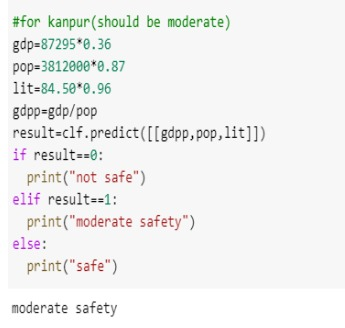
\includegraphics[scale=1.2]{result.jpeg}
            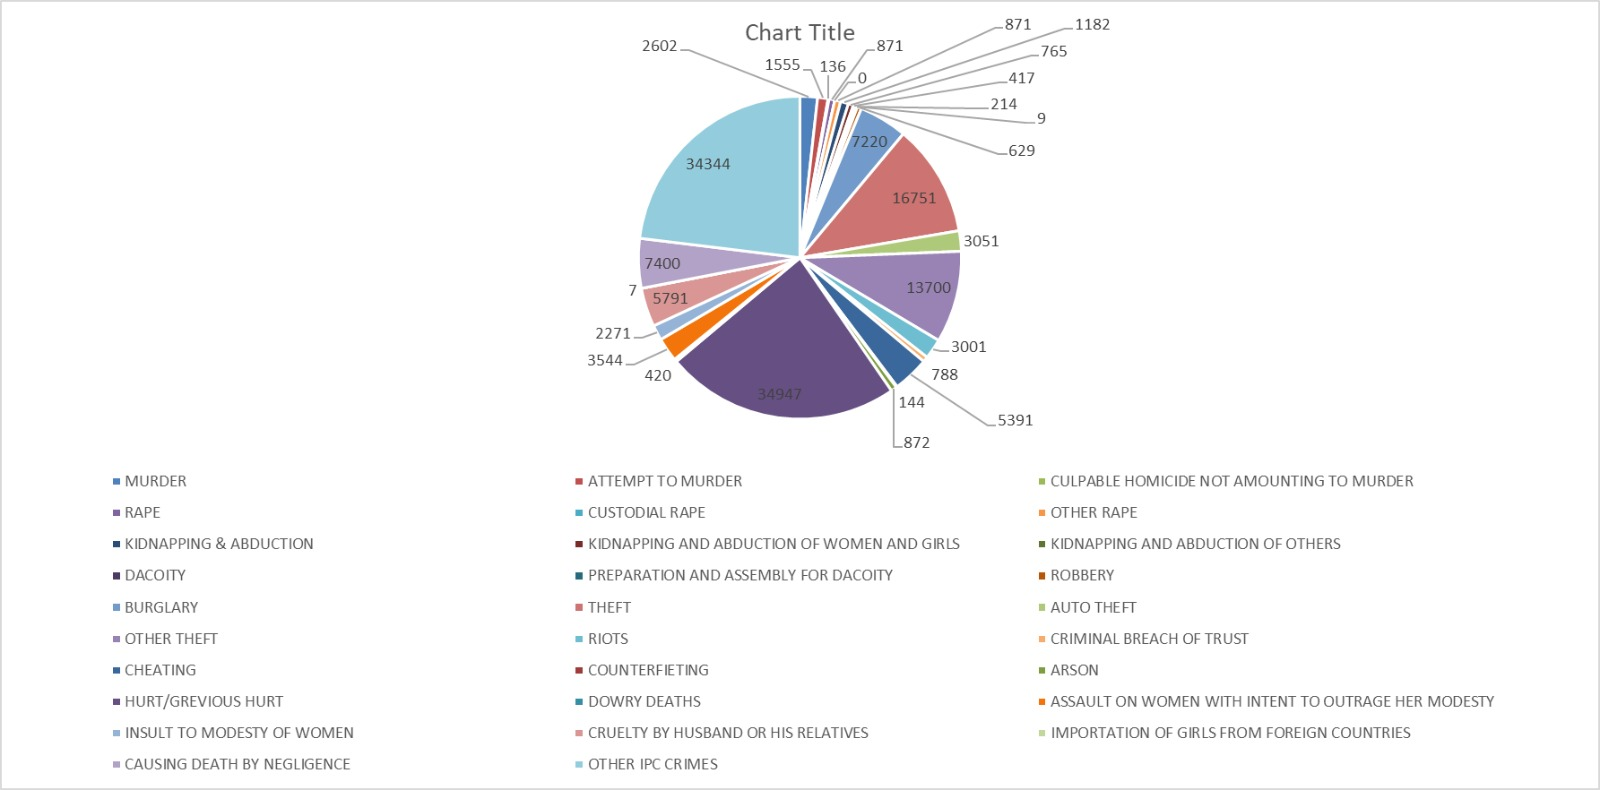
\includegraphics[scale=0.5]{andhra.jpeg}
        \end{tikzfigure}
    }

    \block{7.Conclusion}{
        CRIME GLANCE website for crime prediction is a
        useful resource for comprehending and mitigating
        prospective criminal activity in a variety of contexts. We work to deliver precise insights and
        forecasts to improve public safety by utilising a
        large dataset, sophisticated algorithms, and machine learning techniques. We understand how
        crucial it is to consistently enhance our crime prediction models by incorporating the most recent
        data, enhancing algorithms, and taking user input
        into account. Finally, in the joint effort to create
        safer neighbourhoods, our crime prediction website is a valuable tool. We work to create a future
        where crime rates are lower, people can live more
        independently, and technology can help.

    }


    \block{9.Student Details}{
        Dixa Rai, 9696573707, dixarai20051@gmail.com \\
        Kirti Jha , 6207629808, kirtijha567@gmail.com\\
        Km. Jyoti Sharma, 7388562717, jyotisharmarkt2001@gmail.com \\

    }
    % \block{6.References}{
    %     https://www.customwritings.com/howtowrite/post/research-paper-crime/\\
    %     https://www.sciencegate.app/keyword/2759418\\
    % }



    \column{0.4}%set width of second column

    \block{2. DATA FLOW DIAGRAM }{
        \begin{tikzfigure}
            \\
            \\
            \\
            \\
            \\
            \\
            \\
            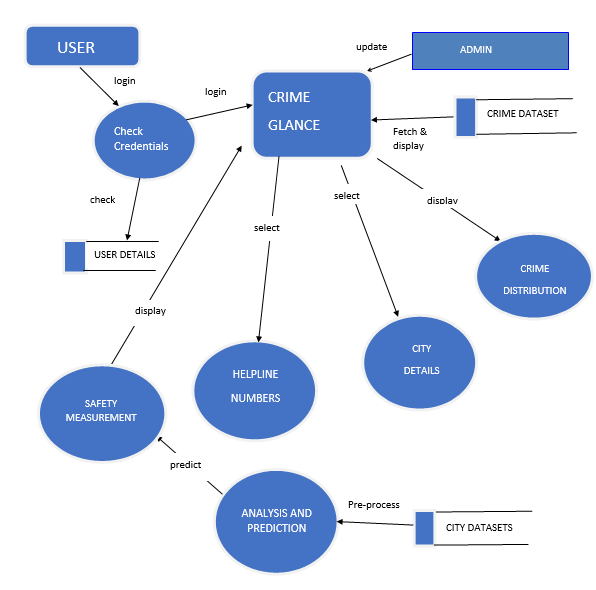
\includegraphics[scale=1]{DFD1Level.png}
        \end{tikzfigure}
    }

    \block{4. ER DIAGRAM}
    {
        \begin{tikzfigure}
            \\
            \\
            \\
            \\
            \\
            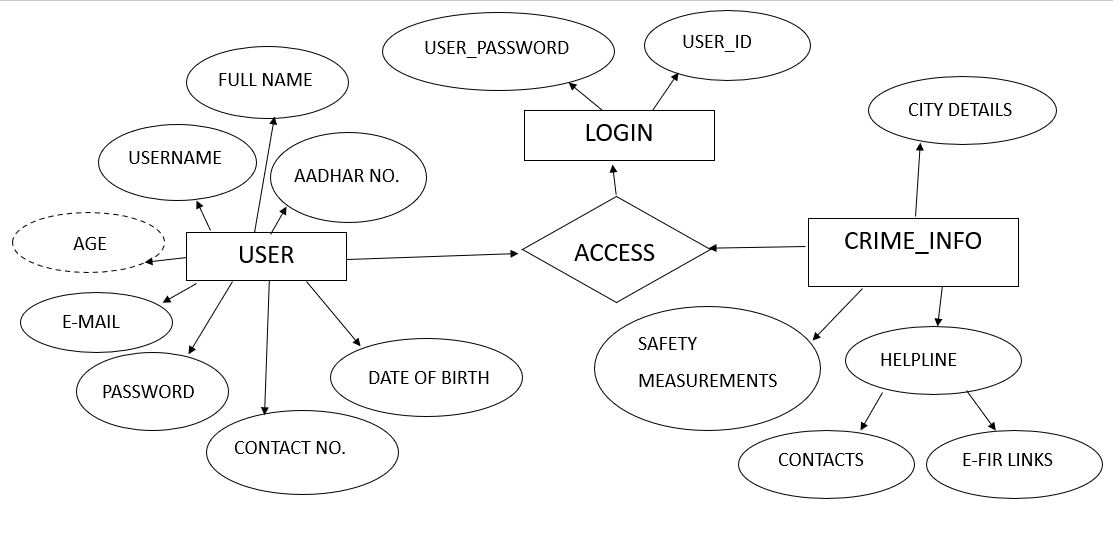
\includegraphics[scale=0.6]{erd.png}
        \end{tikzfigure}
    }

    \block{6. Dashboard}{
        \begin{tikzfigure}
            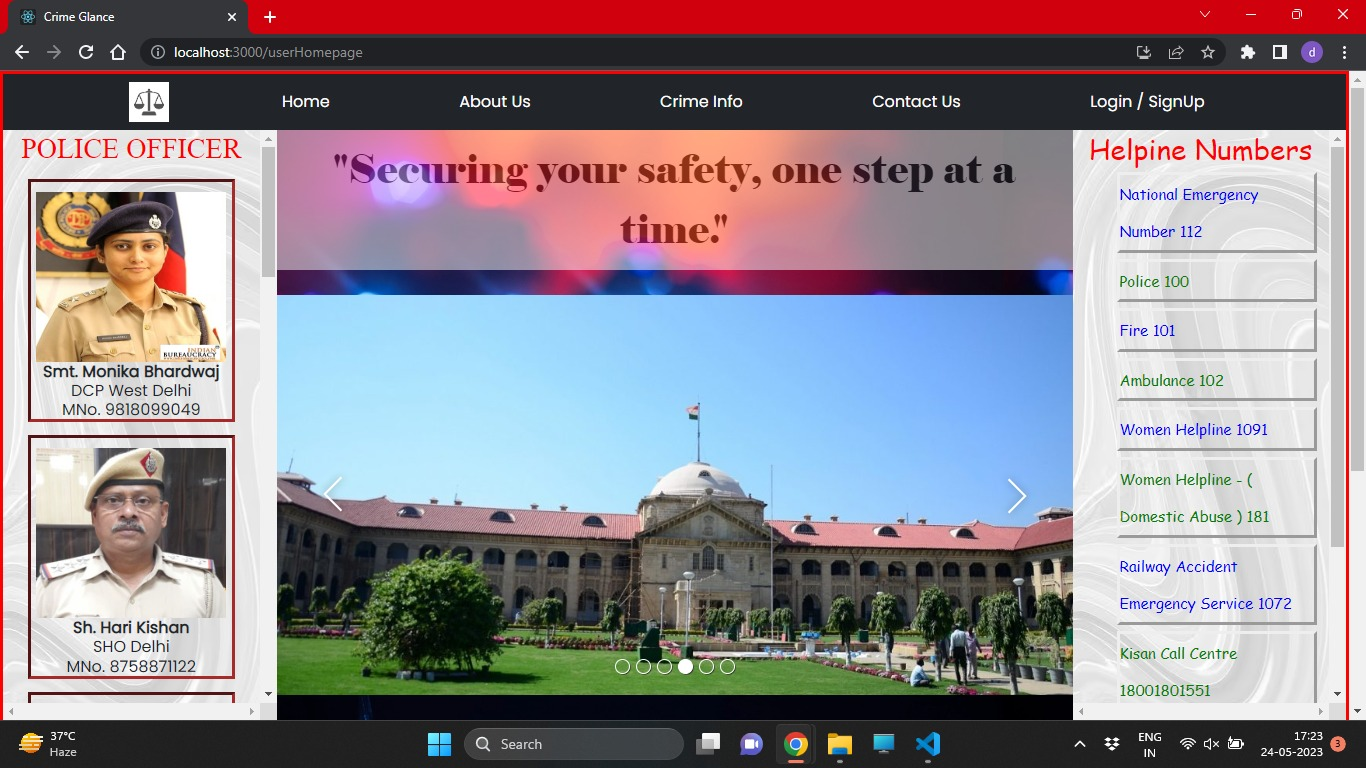
\includegraphics[scale=0.6]{UserHomePage.jpeg}\\
            \\
            \\
        \end{tikzfigure}

        % \begin{tikzfigure}
        %     
\includegraphics[scale=0.5]{emg.jpg}\\
        %     \\
        %     \\
        % \end{tikzfigure}
    }
    \block{8.References}{
        https://www.customwritings.com/howtowrite/post/research-paper-crime/\\
        https://www.sciencegate.app/keyword/2759418\\
    }

    %if necessary, add more columns, adjusting the widths
    %more columns may be necessary in landscape mode

\end{columns}

\end{document}
